% Luonnollisia lukuja käytetään kolmeen eri tarkoitukseen:
% Lukumäärien ilmoittamiseen (kardinaaliluvut)
% Järjestyksen ilmoittamiseen (ordinaaliluvut)
% Indeksointiin ja asioiden nimeämiseen


\subsection*{Luvun käsite}

\termi{luku}{Luku} on käsite, jolla voidaan ilmaista esimerkiksi suuruutta, lukumäärää tai järjestystä. Erityisesti on huomattava, että luku ja \termi{numero}{numero} eivät ole synonyymejä; numero on yksittäinen lukujärjestelmän merkki.

\begin{esimerkki}
	Luku $715531$ koostuu numeroista 7, 1, 5, 5, 3 ja 1.
	
	Luku $9$ koostuu ainoastaan vastaavasta numeromerkistä 9.
\end{esimerkki}

Englannin kielen sana \textit{number} voi viitata sekä numeroon että lukuun. Sana \textit{digit} tarkoittaa pelkästään yhtä numeromerkkiä. Ruotsiksi luku on \textit{tal}, lukumäärä \textit{antal} ja numeroa tai lukumäärää tarkoittamatonta numeroyhdistelmää kuvaa suomen kielen tapaan sana \textit{nummer}.


%Luvulla on aina suuruus mutta numerolla ei välttämättä ole. Esimerkiksi arkipäivän käsitteet postinumero ja puhelinnumero eivät ole lukuja, vaikka niissä numeroita yhdistelläänkin. Emme voi esimerkiksi sanoa, onko postinumero 00950 jollakin tapaa merkitykseltään suurempi kuin postinumero 00900.

Joskus numerosarjoja ei tulkita minkään asian suuruudeksi tai lukumääräksi, vaan ne ovat vain joitain asioita koodaavia lukuja tai merkkijonoja. Esim. postinumero 00900 merkitsee postinkantajalle tiettyä aluetta jolle postia jaetaan. Tietokoneiden ASCII-merkkijärjestelmässä puolestaan luku 125 merkitsee kirjainta U. %vaihtoehtoinen edelliselle kappaleelle. Minusta esim. ASCII-koodeja voidaan sanoa luvuiksi pikemminkin kuin pelkiksi merkkijonoiksi (tätä vahvistaa että sille koodeille on olemassa ekvivalentit esitysmuodot sekä binääri-, oktaali-, kymmen- että heksadesimaalilukujärjestelmissä). -Jouni


\termi{tuhaterotin}{Tuhaterottimena} käytetään suomenkielisessä tekstissä välilyöntiä, ei pilkkua tai pistettä.
\termi{desimaalierotin}{Desimaalierotin} puolestaan on suomenkielisessä tekstissä pilkku, ei piste kuten yhdysvaltalaisissa laskimissa.

%\begin{esimerkki}
%tuhansien erottelu, yhdysvaltalaisessa kirjassa merkintä \$ 1,000.50 tarkoittaa tuhatta dollaria ja 50 senttiä.
%\end{esimerkki}

Matematiikassa lukuja merkitään usein kirjaimilla tai muilla symboleilla. Tästä on se etu, että kirjain voi tarkoittaa mitä lukua tahansa, joten kirjainten avulla pystytään ilmaisemaan kaikille luvuille päteviä yleisiä sääntöjä tarvitsematta välittää siitä, mikä luku johonkin paikkaan kuuluu. Esimerkiksi voimme sanoa, että kaikille luvuille $x$ ja $y$ (ainakin sellaisille, joita lukion matematiikassa käsitellään) pätee $x+y=y+x$. Tämä on paljon helpompaa kuin luetella (äärettömän monta tapausta) esim. $2+3=3+2$, $2+4=4+2$, $3+4=4+3$, $2+5=5+2$, jne.

Yleensä samalla kirjaimella tarkoitetaan samassa asiayhteydessä aina samaa lukua.
Esimerkiksi edellisessä esimerkissä $x$ tarkoittaa samaa lukua yhtälön kummallakin puolella. $y$ tarkoittaa myös jotain lukua joka on sama yhtälön kummallakin puolella. $y$ voi tarkoittaa eri lukua kuin $x$, mutta ei välttämättä. On myös mahdollista, että $x$ ja $y$ voivat tarkoittaa samaa lukua. Siispä yllä mainittu sääntö kertoo myös, että $2+2=2+2$. 

%Laskea-verbin kaksi merkitystä

Kirjaimia, joiden lukuarvo voi vaihdella, on tapana kutsua \termi{muuttuja}{muuttujiksi}\label{muuttuja} ja sellaisia,
joiden lukuarvon ajatellaan pysyvän muuttumattomana, on tapana kutsua \termi{vakio}{vakioiksi}.


\subsection*{Luonnolliset luvut}

%Lukuja on tapana luokitella seuraavasti.
%
%Lukumääriä tai järjestystä esittävät luvut $0, 1, 2, 3, \ldots$ muodostavat
%\termi{luonnollinen luku}{luonnollisten lukujen} joukon $\nn$.
%Toisinaan nollaa ei pidetä luonnollisena lukuna.
%Joukkoja merkitään listaamalla niiden alkiot aaltosuluissa, eli merkitään
%\[\nn=\{0, 1, 2, 3, \ldots \} \]
%
%Kun luonnollisten lukujen joukkoa täydennetään luonnollisten lukujen vastaluvuilla, saadaan \termi{kokonaisluku}{kokonaislukujen} joukko $\zz$.
%\[\zz=\{\ldots, -3, -2, -1, 0, 1, 2, 3, \ldots \} \]

\termi{luonnolliset luvut}{Luonnolliset luvut} ovat lukuja, joita voidaan käyttää lukumäärän ilmaisemiseen.
Luonnollisten lukujen joukkoa merkitään kirjaimella $\nn$ ja niihin katsotaan kuuluvan luvut 0, 1, 2, 3, jne.
Matematiikan kielellä tämä on usein tapana ilmaista seuraavanlaisella merkinnällä: \[\nn = \{0, 1, 2, 3, \ldots\}\]

Luvun kuulumista johonkin joukkoon voidaan merkitä symbolilla $\in$,
esimerkiksi $2 \in \nn$. Jos luku ei kuulu johonkin joukkoon, merkitään vastaavasti $\notin$, esimerkiksi
$-2 \notin \nn$.

Tässä kirjasarjassa katsotaan, että nolla on myös luonnollinen luku. Joissain muissa lähteissä saatetaan kuitenkin
tarkoittaa luonnollisilla luvuilla joukkoa $\mathbb Z_{>0}~=~\{1, 2, 3, \ldots\}$ jota kutsutaan myös positiivisten kokonaislukujen joukoksi. %(myös positiiviset) kokonaisluvut ovat joukko-opillisesti rakennettuna ihan erilaisia otuksia kuin luonnolliset luvut...

Luonnollisille luvuille $m$ ja $n$ on määritelty yhteenlasku $m + n$, esimerkiksi $5 + 3 = 8$.

Luonnollisten lukujen kertolasku määritellään peräkkäisinä yhteenlaskuina

\[5 \cdot 3 = 5 + 5 + 5 = 3 + 3 + 3 + 3 + 3.\]

tai yleisesti kirjaimia käyttäen

\laatikko{ \[m \cdot n = \underbrace{m + m + \ldots + m}_{n\text{ kpl}} = \underbrace{n + n + \ldots + n}_{m\text{ kpl}}.\] }

Nollalla kertomisen ajatellaan olevan ''tyhjä yhteenlasku'' eli nolla:
\laatikko{ \[0 \cdot m = 0\] }

%Luonnollisten lukujen $m$ ja $n$ erotus määritellään yhteenlaskun avulla:
%$m-n$ on luku $k$, jolle $k + n = m$. Kahden luonnollisen luvun erotus
%ei kuitenkaan aina ole luonnollinen luku, esimerkkinä $3 - 5$.
%Ratkaisemme ongelman määrittelemällä kullekin luonnolliselle
%luvulle vastaluvun.

\subsection*{Kokonaisluvut}

Peruskoulun matematiikasta tutuista laskutoimituksista yhteenlasku ja kertolasku ovat ainoat,
joilla voidaan laskea niin, että pysytään luonnollisten lukujen sisällä. Esimerkiksi vähennyslaskua
$3-5$ ei voida laskea luonnollisten lukujen joukossa. Jotta vähennyslasku olisi kaikille luvuille
mahdollinen, on keksitty niin sanottu vastaluvun käsite. Vastaluku määritellään seuraavasti:

\laatikko{ Jokaisella luvulla $n$ on vastaluku $-n$, jolle pätee $n+(-n)=0$. }

Esimerkiksi luvun $2$ vastaluku on $-2$. Yllä olevan määritelmän mukaan, kun luku lasketaan yhteen vastalukunsa kanssa, saadaan tulokseksi $0$. Esimerkiksi $2+(-2)=0$. Vastaavasti luvun $-2$ vastaluku on sellainen luku, joka laskettuna yhteen luvun $-2$ kanssa antaa luvun $0$. Tämä on tietysti $2$, koska $-2+2=0$. Näin voidaan huomata, että $-(-2)=2$. Yleisesti pätee

\laatikko{$$-(-a)=a\text{.}$$}

Tätä kutsutaan peilaukseksi.

Luonnolliset luvut ja niiden vastaluvut muodostavat yhdessä \termi{kokonaisluvut}{kokonaislukujen} joukon

\[\zz = \{\ldots, -2, -1, 0, 1, 2, \ldots\},\] jota voidaan havainnollistaa \termi{lukusuora}{lukusuoran} avulla

\begin{kuva}
	lukusuora.pohja(-4,4,12)
	lukusuora.piste(-3, "$-3$")
	lukusuora.piste(-2,"$-2$")
	lukusuora.piste(-1,"$-1$")
	lukusuora.piste(0,"$0$")
	lukusuora.piste(1,"$1$")
	lukusuora.piste(2,"$2$")
	lukusuora.piste(3,"$3$")
\end{kuva}

%\begin{center}
%\begin{lukusuora}{-4}{4}{10}
%\lukusuorapiste{-3}{}
%\lukusuorapiste{-2}{}
%\lukusuorapiste{-1}{}
%\lukusuorapiste{0}{}
%\lukusuorapiste{1}{}
%\lukusuorapiste{2}{}
%\lukusuorapiste{3}{}
%\lukusuoraalanimi{-3}{$-3$}
%\lukusuoraalanimi{-2}{$-2$}
%\lukusuoraalanimi{-1}{$-1$}
%\lukusuoraalanimi{0}{$0$}
%\lukusuoraalanimi{1}{$1$}
%\lukusuoraalanimi{2}{$2$}
%\lukusuoraalanimi{3}{$3$}
%
%\end{lukusuora}
%\end{center}

Kun käytämme kokonaislukuja, voidaan kahden luvun erotus määritellä
yhteenlaskun ja vastaluvun avulla yksinkertaisesti:

\laatikko{
\[m-n = m+(-n)\]
}

\subsection*{Rationaaliluvut}

Peruskoulussa opituista laskutoimituksista yhteenlasku, vähennyslasku ja kertolasku ovat sellaisia, joilla voidaan laskea niin, että pysytään kokonaislukujen sisällä. Samoin esimerkiksi laskusta $8:4$ tulee tulokseksi kokonaisluku $2$. Sen sijaan esimerkiksi laskutoimituksella $8:3$ ei ole tulosta kokonaislukujen joukossa. Tätä varten on otettu käyttöön rationaaliluvun käsite.

\termi{rationaaliluku}{Rationaaliluvulla} tarkoitetaan lukua, joka voidaan esittää kahden kokonaisluvun osamääränä. Esimerkiksi $\frac{2}{3}$ on rationaaluku, samoin $0,25=\frac{1}{4}$. Myös kaikki kokonaisluvut ovat rationaalilukuja, sillä ne voidaan esittää osamäärinä: esimerksi $5=\frac{5}{1}$. Rationaalilukujen joukkoa merkitään symbolilla $\qq$. \[\qq= \text{ rationaalilukujen joukko} \]    


\subsection*{Reaaliluvut}

Kaikki käyttämämme luvut eivät ole edes rationaalilukuja. Esimerkiksi peruskoulussa on käytetty lukua $\pi$, joka kuvaa ympyrän kehän pituuden suhdetta ympyrän halkaisijaan. Lukua $\pi$ ei voida esittää kahden kokonaisluvun osamääränä, joten se ei ole rationaaliluku.

Toinen esimerkki luvusta, joka ei ole rationaaliluku on $\sqrt{2}$. $\sqrt{2}$ tarkoittaa sellaista positiivista lukua, joka kerrottuna itsellään on 2. Se tulee vastaan esimerksi suorakulmaisessa kolmiossa, jonka kateetit ovat pituudeltaan 1. (Neliöjuuren käsitteestä puhutaan tarkemmin tämän kirjan luvussa \ref{neliojuuri}.)

\begin{kuva}
	skaalaa(4)

	A=(0,0)
	B=(0,1)
	C=(1,0)
	D=(0.1,0.1)
	E=(0,0.1)
	F=(0.1,0)

	geom.jana(B,A,"$1$")
	geom.jana(C,B,r"$\sqrt{2}$")
	geom.jana(A,C,"$1$")
	geom.jana(E,D)
	geom.jana(D,F)
\end{kuva}

Sellaisia lukuja, kuten $\pi$ ja $\sqrt{2}$, joita ei voida esittää kahden kokonaisluvun osamääränä,
sanotaan \termi{irrationaaliluku}{irrationaaliluvuiksi}. Rationaaliluvut ja irrationaaliluvut muodostavat
yhdessä \termi{reaaliluku}{reaalilukujen} joukon $\rr$.

Reaalilukujen ominaisuuksista kerrotaan lisää luvussa \ref{reaaliluvut}.

Seuraavassa taulukossa on yhteenveto lukiokursseilla käytettävistä lukualueista:
\begin{center}\begin{tabular}{l|c|l}
Joukko & Symboli & Mitä ne ovat\\
\hline
Luonnolliset luvut & $\nn$ &
Luvut $0$, $1$, $2$, $3$, $\ldots$ \\
Kokonaisluvut & $\zz$ & Luvut $\ldots$ $-2$, $-1$, $0$, $1$, $2$ $\ldots$ \\ 
Rationaaliluvut & $\qq$ & Luvut, jotka voidaan esittää
murtolukuna \\
Reaaliluvut & $\rr$ & Kaikki lukusuoran luvut \\
& & eli kaikki desimaaliluvut
\end{tabular} \end{center} 

Joukot $\nn$, $\zz$, $\qq$ ja $\rr$ ovat sisäkkäisiä. Kaikki luonnolliset luvut ovat myös kokonaislukuja,
kaikki kokonaisluvut ovat myös rationaalilukuja ja kaikki rationaaliluvut ovat myös reaalulukuja.

\begin{tikzpicture}[line cap=round,line join=round,>=triangle 45,x=0.5cm,y=0.5cm]
\clip(-7.4,-8.8) rectangle (16.8,8.6);
\draw [rotate around={0.5:(2.2,0)}] (2.2,0) ellipse (1.1cm and 0.9cm);
\draw [rotate around={-0.8:(2.5,0)}] (2.5,0) ellipse (2cm and 1.6cm);
\draw [rotate around={-0.8:(2.5,0)}] (2.5,0) ellipse (2.9cm and 2.6cm);
\draw (2,1.5) node[anchor=north west] {$\nn$};
\draw (4.0,2.7) node[anchor=north west] {$\zz$};
\draw (5.5,3.9) node[anchor=north west] {$\qq$};
%\draw (6.6,-4.6) node[anchor=north west] {{\scriptsize Irrationaaliluvut}};
\draw (9.5,6.4) node[anchor=north west] {$\rr$};
\draw [rotate around={0.5:(4.4,0)}] (4.4,0) ellipse (5cm and 4.2cm);
%\draw [rotate around={18.2:(7.9,-5.4)}] (7.9,-5.4) ellipse (2.7cm and 0.6cm);
\draw (0.8,1.6) node[anchor=north west] {$1$};
\draw (1,-0.4) node[anchor=north west] {$5$};
\draw (2.4,-0.2) node[anchor=north west] {$101$};
\draw (4.8,0.7) node[anchor=north west] {$-5$};
\draw (1.2,-1.7) node[anchor=north west] {$0$};
\draw (1.2,3.1) node[anchor=north west] {$-14$};
%\draw (4.1,-1) node[anchor=north west] {$75$};
\draw (4.2,-2.8) node[anchor=north west] {$-\frac{1}{3}$};
\draw (6.6,1.4) node[anchor=north west] {$2\frac{1}{2}$};
\draw (-1.6,0.9) node[anchor=north west] {$-3$};
%\draw (0.4,-3.1) node[anchor=north west] {$-4$};
\draw (2.4,4.7) node[anchor=north west] {$2,6$};
\draw (-1.3,4.1) node[anchor=north west] {$\frac{5}{7}$};
\draw (-2.7,-1) node[anchor=north west] {$0,1$};
\draw (5.5,-5.9) node[anchor=north west] {$\pi$};
\draw (9.1,-3) node[anchor=north west] {$\sqrt[]{2}$};
%\draw (6,-4.7) node[anchor=north west] {$-\frac{\pi}{2}$};
%\draw (9.8,1.6) node[anchor=north west] {$\frac{5}{2}$};
\draw (10.5,3) node[anchor=north west] {$\frac{1}{\sqrt{2}}$};
%\draw (4.4,7.3) node[anchor=north west] {$3$};
\draw (-0.1,-5.3) node[anchor=north west] {$\sqrt{15}$};
%\draw (-4.9,1.5) node[anchor=north west] {$-5$};
\draw (11.8,-0.9) node[anchor=north west] {$-\frac{\pi}{2}$};
\draw (-0.6,6.8) node[anchor=north west] {$0,10110111011110\ldots$};
%\draw (-3.7,-3) node[anchor=north west] {$-3$};
\end{tikzpicture}

Lukualueiden ominaisuudet tulevat tarkemmin esille tämän kirjan myöhemmissä luvuissa.

Lukualueita voidaan laajentaa lisää vielä reaaliluvuistakin - - esimerkiksi \termi{kompleksiluvut}{kompleksiluvuiksi},
jotka voidaan esittää tason pisteinä. Kompleksilukuja merkitään kirjaimella $\cc$. Kompleksiluvut eivät
kuulu lukion oppimäärään, mutta niitä tarvitaan muun muassa insinöörialoilla yliopistoissa
ja ammattikorkeakouluissa. Esimerkiksi vaihtosähköpiirien analyysissä, signaalinkäsittelyssä ja
säätötekniikassa käytetään runsaasti kompleksilukuja. Kompleksiluvut ovat tärkeitä myös matematiikan
tutkimuksessa itsessään. Tässä kirjassa niihin ei kuitenkaan perehdytä tarkemmin.

% === SIISTITTÄVÄ PÄTKÄ ALKAA ===

\subsection*{Laskutoimitukset}
Peruskoulusta tuttuja laskutoimituksia ovat muunmuassa yhteen-, vähennys-, kerto- ja jakolasku. Huomaa, että joitakin laskutoimituksia
voidaan merkitä useilla eri tavoilla:

\begin{center}\begin{tabular}{l|l}
Laskutoimitus & Merkintä\\
\hline
Yhteenlasku & $+$ \\
Vähennyslasku & $-$ \\
Kertolasku & $ \times $  $ \ast $  $ \cdot $ \\
Jakolasku & $:$ $/$ $-$ (jakoviivana) \\
\end{tabular} \end{center} 

Laskimista tuttua symbolia $\div$ ei tulisi käyttää käsinkirjoitetussa lausekkeissa. Jakoviivan ylä- ja alapuolilla olevat 
pisteet kuvaavat murtolukuesityksen osoittajaa ja nimittäjää. Siis esimerkiksi laskimeen näppäilty ``$4\div2$'' vastaa jakoviivan avulla merkittyä
murtolukuesitystä $\frac{4}{2}$.

\laatikko{
\begin{itemize}
\item{$\text{yhteenlaskettava}+\text{yhteenlaskettava}=\text{summa}$}
\item{$\text{vähennettävä}-\text{vähentäjä}=\text{erotus}$}
\item{$\text{tekijä} \cdot \text{tekijä}=\text{tulo}$}
\item{$\text{jaettava} :\text{jakaja}=\text{osamäärä}$}
\end{itemize}
}

Yllä on lueteltu peruslaskutoimituksiin osallistuville luvuille annetut nimitykset. Huomaa, että yhteen- ja kertolaskussa laskutoimitukseen 
osallistuvia lukuja nimitetään samalla tavalla. Tämä kertoo yhteen- ja kertolaskun vaihdannaisuudesta. Näissä laskutoimituksissa
lukujen järjestyksellä ei siis ole väliä.

Kuten tullaan näkemään, kerto- ja jakolasku määritellään yhteenlaskun avulla.

\subsection*{Yhteen- ja vähennyslaskun merkkisäännöt}

Vähennyslasku määriteltiin kokonaislukujen yhteydessä vastaluvun lisäämiseksi:

\[m-n = m+(-n)\]

Tämän perusteella voidaan myös päätellä, mitä tapahtuu, kun vähennettävä luku onkin negatiivinen. Esimerkiksi:

\begin{align*}
&8-(-5)&\quad\quad\quad\textrm{Muutetaan vähennyslasku vastaluvun lisäämiseksi}\\
= &8+(-(-5))&\quad\quad\quad\textrm{$-(-5)$ tarkoittaa $-5$:n vastalukua, joka on 5.}\\
= &8+5
\end{align*}

Tähän ideaan perustuvat seuraavat merkkisäännöt yhteen- ja vähennyslaskulle:

\laatikko{
\begin{itemize}
\item{$a+(+b)=a+b$}
\item{$a+(-b)=a-b$}
\item{$a-(+b)=a-b$}
\item{$a-(-b)=a+b$}
\end{itemize}
}

Tämä asia ilmaistaan usein sanomalla, että kaksi peräkkäistä '$-$'-merkkiä kumoavat toisensa.


%Seuraavassa kommentoituna taulukoitu versio lukusuorista.

%\begin{luoKuva}{yhteenlasku1}
%	lukusuora.pohja(-4,14,4,n=2, varaa_tila = False)
%	with vari("red"):
%		lukusuora.vali(0,5,i=1)
%		lukusuora.vali(8,13,i=2)
%	with vari("blue"): lukusuora.vali(0,8,i=2)
%	lukusuora.piste(0,"$0$")
%	lukusuora.piste(5,"$5$",1)
%	lukusuora.piste(8,"$8$",2)
%	lukusuora.piste(13,"$13$",2)
%\end{luoKuva}
%\begin{luoKuva}{yhteenlasku2}
%	lukusuora.pohja(-4,14,4,n=2)
%	with vari("red"):
%		lukusuora.vali(0,5,i=1)
%		lukusuora.vali(8,13,i=2)
%	with vari("blue"): lukusuora.vali(0,8,i=2)
%	lukusuora.piste(0,"$0$")
%	lukusuora.piste(5,"$5$",1)
%	lukusuora.piste(8,"$8$",2)
%	lukusuora.piste(13,"$13$",2)
%\end{luoKuva}
%\begin{luoKuva}{yhteenlasku3}
%	lukusuora.pohja(-4,14,4,n=2)
%	with vari("red"):
%		lukusuora.vali(0,5,i=2)
%	with vari("blue"): lukusuora.vali(-3,5,i=1)
%	lukusuora.piste(0,"$0$",2)
%	lukusuora.piste(5,"$5$")
%	lukusuora.piste(-3,"$-3$",1)
%\end{luoKuva}
%\begin{luoKuva}{yhteenlasku4}
%	lukusuora.pohja(-4,14,4,n=2)
%	with vari("red"):
%		lukusuora.vali(0,5,i=2)
%	with vari("blue"): lukusuora.vali(-3,5,i=1)
%	lukusuora.piste(0,"$0$",2)
%	lukusuora.piste(5,"$5$")
%	lukusuora.piste(-3,"$-3$",1)
%\end{luoKuva}
%\begin{luoKuva}{yhteenlasku5}
%	lukusuora.pohja(-4,14,4,n=2)
%	with vari("red"):
%		lukusuora.vali(0,5,i=1)
%		lukusuora.vali(8,13,i=2)
%	with vari("blue"): lukusuora.vali(0,8,i=2)
%	lukusuora.piste(0,"$0$")
%	lukusuora.piste(5,"$5$",1)
%	lukusuora.piste(8,"$8$",2)
%	lukusuora.piste(13,"$13$",2)
%\end{luoKuva}
%\begin{tabular}{|p{4.0cm}|c|}
%\hline
% ${\color{red}5}+{\color{blue}8}=13$ & \naytaKuva{yhteenlasku1}  \\
%\hline
% ${\color{red}5}+({\color{blue}+8})=13$ & \naytaKuva{yhteenlasku2}  \\
%\hline
% ${\color{red}5}-({\color{blue}+8})=-3$ & \naytaKuva{yhteenlasku3}  \\
%\hline
%${\color{red}5}+({\color{blue}-8})=-3$ & \naytaKuva{yhteenlasku4} \\
%\hline
%${\color{red}5}-({\color{blue}-8})=13$ & \naytaKuva{yhteenlasku5}  \\
%\hline
%\end{tabular}

    Negatiivisten ja positiivisten lukujen yhteen- ja vähennyslaskut voidaan helposti tulkita lukusuoran avulla.
    
    % tässä on vähän kyseenalaista käyttää sekaisin sanallista ja numeerista esitystä

    $5+8$ ''viiteen lisätään kahdeksan''
    
\begin{center}
\begin{kuva}
	lukusuora.pohja(-4,14,12,n=2)
	with vari("red"):
		lukusuora.vali(0,5,i=1)
		lukusuora.vali(8,13,i=2)
	with vari("blue"): lukusuora.vali(0,8,i=2)
	lukusuora.piste(0,"$0$")
	lukusuora.piste(5,"$5$",1)
	lukusuora.piste(8,"$8$",2)
	lukusuora.piste(13,"$13$",2)
\end{kuva}
%      \begin{lukusuora}{-1}{14}{14}
%        %\lukusuoranuolialas{5}{13}
%        %\lukusuoranuolialas{0}{8}
%        {\color{red} \lukusuoravaliss{0}{5}{$0$}{$5$}}
%        \lukusuorauusi
%        {\color{red} \lukusuoravaliss{8}{13}{$8$}{${\color{black}13}$}}
%        {\color{blue} \lukusuoravaliss{0}{8}{$0$}{$8$}}
%       \end{lukusuora}
       ${\color{red}5}+{\color{blue}8}=13$
\end{center}
   
    $5+(+8)$ ''viiteen lisätään plus kahdeksan''
    
    $+8$ tarkoittaa samaa kuin $8$. '$+$'-merkkiä käytetään luvun edessä silloin, kun halutaan korostaa, että kyseessä on nimenomaan positiivinen luku.
    
%säädetään kuva vähän irti tuosta edeltävästä tektistä
%\vspace{0.3cm}     
    
\begin{center}
\begin{kuva}
	lukusuora.pohja(-4,14,12,n=2)
	with vari("red"):
		lukusuora.vali(0,5,i=1)
		lukusuora.vali(8,13,i=2)
	with vari("blue"): lukusuora.vali(0,8,i=2)
	lukusuora.piste(0,"$0$")
	lukusuora.piste(5,"$5$",1)
	lukusuora.piste(8,"$8$",2)
	lukusuora.piste(13,"$13$",2)
\end{kuva}
%          \begin{lukusuora}{-1}{14}{14}
%        {\color{red} \lukusuoravaliss{0}{5}{$0$}{$5$}}
%        \lukusuorauusi
%        {\color{red} \lukusuoravaliss{8}{13}{$8$}{${\color{black}13}$}}
%        {\color{blue} \lukusuoravaliss{0}{8}{$0$}{$8$}}
%       \end{lukusuora}
       ${\color{red}5}+({\color{blue}+8})=13$
\end{center}
    
    $5-(+8)$ ''viidestä vähennetään $+8$''
    
    Tämä tarkoittaa samaa kuin $5-8$. Lukusuoralla siis liikutaan 8 pykälää taaksepäin.

%säädetään kuva vähän irti tuosta edeltävästä tektistä
\vspace{0.3cm}     
    
\begin{center}
\begin{kuva}
	lukusuora.pohja(-4,14,12,n=2)
	with vari("red"):
		lukusuora.vali(0,5,i=2)
	with vari("blue"): lukusuora.vali(-3,5,i=1)
	lukusuora.piste(0,"$0$",2)
	lukusuora.piste(5,"$5$")
	lukusuora.piste(-3,"$-3$",1)
\end{kuva}
%              \begin{lukusuora}{-4}{8}{14}
%        {\color{blue} \lukusuoravaliss{-3}{5}{\color{black}$-3$}{$5$}}
%        \lukusuorauusi
%%        {\color{red} \lukusuoravaliss{8}{13}{$8$}{${\color{black}13}$}}
%        {\color{red} \lukusuoravaliss{0}{5}{$0$}{$5$}}
%       \end{lukusuora}
       ${\color{red}5}-({\color{blue}+8})=-3$
\end{center}


%lukiolaiset pitivät näitä epäselvinä kuvina
%[Joonas]: Tarvittaisiin vierekkäin olevat nuolet
    
Mitä tapahtuu, kun lisätään negatiivinen luku? Kun lukuun lisätään $1$, se kasvaa yhdellä. Kun lukuun lisätään $0$, se ei kasva lainkaan. Kun lukuun lisätään negatiivinen luku, esimerkiksi $-1$, on luonnollista ajatella, että se pienenee. Tällä logiikalla negatiivisen luvun lisäämisen pitäisi siis pienentää alkuperäistä lukua. Juuri näin vähennyslasku määritellään: $5+(-8)$ on yhtä suuri kuin $5-8$.
    
\vspace{0.3cm}     
\begin{center}
\begin{kuva}
	lukusuora.pohja(-4,14,12,n=2)
	with vari("red"):
		lukusuora.vali(0,5,i=2)
	with vari("blue"): lukusuora.vali(-3,5,i=1)
	lukusuora.piste(0,"$0$",2)
	lukusuora.piste(5,"$5$")
	lukusuora.piste(-3,"$-3$",1)
\end{kuva}
%                 \begin{lukusuora}{-4}{8}{14}
%        {\color{blue} \lukusuoravaliss{-3}{5}{\color{black}$-3$}{$5$}}
%        \lukusuorauusi
%%        {\color{red} \lukusuoravaliss{8}{13}{$8$}{${\color{black}13}$}}
%        {\color{red} \lukusuoravaliss{0}{5}{$0$}{$5$}}
%       \end{lukusuora}
       ${\color{red}5}+({\color{blue}-8})=-3$
\end{center}
    
    
    $5-(-8)$ ''viidestä vähennetään miinus kahdeksan''
    
    Negatiivisen luvun lisääminen on vastakohta positiivisen luvun lisäämiselle. Tällöin on luonnollista, että negatiivisen luvun vähentäminen on vastakohta positiivisen luvun vähentämiselle. Koska positiivisen luvun vähentäminen pienentää lukua, pitäisi negatiivisen luvun vähentämisen kasvattaa lukua. Lasku $5-(-8)$ tarkoittaa siis samaa kuin $5+8$.
\vspace{0.3cm}     
        
\begin{center}
\begin{kuva}
	lukusuora.pohja(-4,14,12,n=2)
	with vari("red"):
		lukusuora.vali(0,5,i=1)
		lukusuora.vali(8,13,i=2)
	with vari("blue"): lukusuora.vali(0,8,i=2)
	lukusuora.piste(0,"$0$")
	lukusuora.piste(5,"$5$",1)
	lukusuora.piste(8,"$8$",2)
	lukusuora.piste(13,"$13$",2)
\end{kuva}
%    \begin{lukusuora}{-1}{14}{14}
%        {\color{red} \lukusuoravaliss{0}{5}{$0$}{$5$}}
%        \lukusuorauusi
%        {\color{red} \lukusuoravaliss{8}{13}{$8$}{${\color{black}13}$}}
%        {\color{blue} \lukusuoravaliss{0}{8}{$0$}{$8$}}
%       \end{lukusuora}
       ${\color{red}5}-({\color{blue}-8})=13$
\end{center}


%Koska $+b-b=0$, yhteen- ja vähennyslasku kumoavat toisensa, eli
%
%\begin{itemize}
%\alakohta{$a+b-b=a$
%\alakohta{$a-b+b=a$
%\end{itemize}



\subsection*{Kertolasku}

    Samaan logiikkaan perustuen on sovittu myös merkkisäännöt positiivisten ja negatiivisten lukujen kertolaskuissa. Kun negatiivinen ja positiivinen luku kerrotaan keskenään, saadaan negatiivinen luku, mutta kun kaksi negatiivista lukua kerrotaan keskenään, saadaan positiivinen luku.

    $3 \cdot 4$ ''kolme kappaletta nelosia''
    
\begin{center}
\begin{kuva}
	lukusuora.pohja(-14,14,12)
	vari("red")
	lukusuora.vali(0,4)
	lukusuora.vali(4,8)
	lukusuora.vali(8,12)
	vari("black")
	lukusuora.piste(0,"$0$")
	lukusuora.piste(4,"$4$")
	lukusuora.piste(8,"$8$")
	lukusuora.piste(12,"$12$")
\end{kuva}
%    \begin{lukusuora}{-1}{14}{14}
%	\color{red} \lukusuoravaliss{0}{4}{$0$}{$4$}
%	\color{red} \lukusuoravaliss{4}{8}{$4$}{$8$}
%	\color{red} \lukusuoravaliss{8}{12}{$8$}{$12$}
%
%      \end{lukusuora}
      $3\cdot {\color{red}4}=12$
\end{center}
    
    $3 \cdot (-4)$ ''kolme kappaletta miinus-nelosia''
    
    
\begin{center}
\begin{kuva}
	lukusuora.pohja(-14,14,12)
	vari("red")
	lukusuora.vali(-4,0)
	lukusuora.vali(-8,-4)
	lukusuora.vali(-12,-8)
	vari("black")
	lukusuora.piste(0,"$0$")
	lukusuora.piste(-4,"$-4$")
	lukusuora.piste(-8,"$-8$")
	lukusuora.piste(-12,"$-12$")
\end{kuva}
%    \begin{lukusuora}{-13}{2}{14}
%	\color{red} \lukusuoravaliss{-12}{-8}{$-12$}{$-8$}
%	\color{red} \lukusuoravaliss{-8}{-4}{$-8$}{$-4$}
%	\color{red} \lukusuoravaliss{-4}{0}{$-4$}{$0$}
%
%      \end{lukusuora}
      $3\cdot ({\color{red}-4})=-12$
\end{center}
    
    $-3 \cdot 4$ ''miinus-kolme nelinkertaistetaan''
    
\begin{center}
\begin{kuva}
	lukusuora.pohja(-14,14,12)
	vari("blue")
	lukusuora.vali(-3,0)
	lukusuora.vali(-6,-3)
	lukusuora.vali(-9,-6)
	lukusuora.vali(-12,-9)
	vari("black")
	lukusuora.piste(0,"$0$")
	lukusuora.piste(-3,"$-3$")
	lukusuora.piste(-6,"$-6$")
	lukusuora.piste(-9,"$-9$")
	lukusuora.piste(-12,"$-12$")
\end{kuva}
%    \begin{lukusuora}{-13}{2}{14}
%	\color{red} \lukusuoravaliss{-12}{-9}{$-12$}{$-9$}
%	\color{red} \lukusuoravaliss{-9}{-6}{$-9$}{$-6$}
%	\color{red} \lukusuoravaliss{-6}{-3}{$-6$}{$-3$}
%	\color{red} \lukusuoravaliss{-3}{0}{$-3$}{$0$}
%
%      \end{lukusuora}
      ${\color{blue}-3}\cdot 4=-12$
\end{center}
    
    $-3 \cdot (-4)$ ''miinus-kolme miinus-nelinkertaistetaan''
    
\begin{center}
\begin{kuva}
	lukusuora.pohja(-14,14,12)
	vari("blue")
	lukusuora.vali(0,3)
	lukusuora.vali(3,6)
	lukusuora.vali(6,9)
	lukusuora.vali(9,12)
	vari("black")
	lukusuora.piste(0,"$0$")
	lukusuora.piste(3,"$3$")
	lukusuora.piste(6,"$6$")
	lukusuora.piste(9,"$9$")
	lukusuora.piste(12,"$12$")
\end{kuva}
%    \begin{lukusuora}{-1}{14}{14}
%	\color{red} \lukusuoravaliss{12}{9}{$12$}{$9$}
%	\color{red} \lukusuoravaliss{9}{6}{$9$}{$6$}
%	\color{red} \lukusuoravaliss{6}{3}{$6$}{$3$}
%	\color{red} \lukusuoravaliss{3}{0}{$3$}{$0$}
%
%      \end{lukusuora}
      ${\color{blue}-3}\cdot (-4)=12$
\end{center}

\subsection*{Jakolasku}
%Lisää visualisointi!

Kun ensin kerrotaan jollain ja sitten jaetaan samalla luvulla, päädytään takaisin siihen
mistä lähdettiin.  Jakolaskujen merkkisäännöt on sovittu niin, että tämä ominaisuus säilyy.
Ne ovat siis samat kuin kertolaskujen merkkisäännöt.

Esimerkiksi haluamme, että $(-12):(-3)\cdot (-3)=-12$. Nyt voimme kysyä, mitä laskun
$(-12):(-3)$ tulokseksi pitäisi tulla, jotta jakolasku ja kertolasku säilyvät toisilleen
käänteisinä, eli mikä luku kerrottuna luvulla $-3$ on $-12$. Kertolaskun merkkisäännöistä
nähdään helposti, että tämän luvun täytyy olla $+4$ eli $4$. Niinpä on
sovittu, että $(-12):(-3)=12:3=4$.

\laatikko{
Kerto- ja jakolaskun merkkisäännöt
\begin{alakohdat}
\alakohta{$a\cdot (-b)=(-a)\cdot b=-(ab)$}
\alakohta{$(-a)\cdot (-b)=a\cdot b=ab$}
\alakohta{$(-a):b=a:(-b)=-\dfrac{a}{b}$}
\alakohta{$(-a):(-b)=a: b=\dfrac{a}{b}$}
\end{alakohdat}
}

\subsection*{Jaollisuus ja tekijöihinjako}
%Omaksi luvukseen?

\laatikko{
	\textbf{Määritelmä 1}
	Kokonaisluku $a$ on jaollinen kokonaisluvulla $b \neq 0$, jos on olemassa kokonaisluku $c$ niin, että $a = b \cdot c$.
	Tällöin sanotaan myös, että $b$ on $a$:n \termi{tekijä}{tekijä}.

	\vspace*{24pt}

	\textbf{Määritelmä 2}
	Luku $a$ on jaollinen luvulla $b \neq 0$, mikäli $\frac{a}{b}$ on kokonaisluku.
	
	Määritelmät ovat yhtäpitäviä.
}
    
\begin{esimerkki}
	\begin{alakohdat}
		\alakohta{Luku $-12$ on jaollinen luvulla $3$, sillä $-12 = 3 \cdot (-4)$.}
		\alakohta{$-12$ ei ole jaollinen luvulla $5$, sillä ei ole kokonaislukua, joka kerrottuna viidellä olisi $12$.}
	\end{alakohdat}
\end{esimerkki}
   
\begin{center}
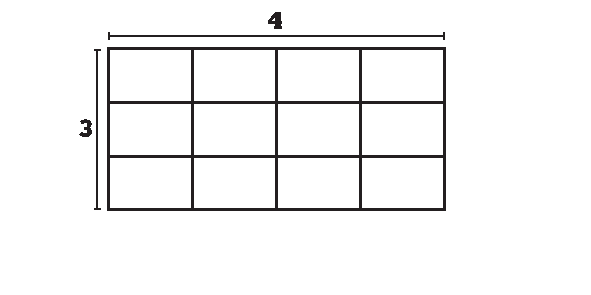
\includegraphics[scale=0.85]{pictures/Kuva2-4-3x4.pdf}
\end{center}
    
Kaikki luvut ovat jaollisia itsellään ja luvulla $1$. Esimerkiksi $7=7 \cdot 1=1 \cdot 7$, joten $7$ on jaollinen luvuilla $1$ ja $7$.
    
\laatikko{
	\termi{alkuluku}{Alkuluku} on ykköstä suurempi kokonaisluku, joka ei ole jaollinen muilla positiivisilla kokonaisluvuilla kuin luvulla $1$ ja itsellään.
}
    
Esimerkiksi luvut 2, 3, 5, 7, 11, 13, 17 ja 19 ovat alkulukuja. Jos luvun tekijä on alkuluku, sitä kutsutaan \termi{alkutekijä}{alkutekijäksi}.
    
\laatikko{
    \textbf{Aritmetiikan peruslause}
	
    Jokainen ykköstä suurempi kokonaisluku voidaan esittää (termien järjestystä lukuunottamatta) yksikäsitteisesti alkulukujen tulona.
	(Jokainen ykköstä suurempi kokonaisluku voidaan jakaa alkutekijöihin (termien järjestystä lukuunottamatta) yksikäsitteisellä tavalla.)
}
    
Aritmetiikan peruslause todistetaan kurssilla Logiikka ja lukuteoria.
    
Esimerkiksi luku $84$ voidaan kirjoittaa muodossa $2\cdot 2\cdot 3\cdot 7$. Havaitaan, että $2$, $3$, ja $7$ ovat kaikki alkulukuja. Aritmetiikan peruslauseen nojalla tiedetään, että tämä on ainoa tapa kirjoittaa $84$ alkulukujen tulona -- mahdollista kerrottavien termien järjestyksen vaihtoa lukuunottamatta.
    
Luvun alkutekijät voi löytää etsimällä luvulle ensin jonkin esityksen kahden luvun tulona. Näiden kahden luvun ei tarvitse olla alkulukuja. Sen jälkeen sama toistetaan näille kahdelle luvulle ja edelleen aina uusille luvuille, kunnes jäljellä on vain alkulukuja.
